\chapter{Interaktionsdesign}
\section{Analyse}
In diesem Abschnitt soll analysiert werden, wie die möglichen Interaktionen gestaltet sind. Werden die Designprinzipien Normans (Kap. \ref{sec:interactionDesign}) nicht hinreichend erfüllt, lässt dies auf ein zu behebendes Problem der User-Experience schließen.
Da es sich bei \textit{FalkoFX} um eine bestehende Anwendung in der Entwicklungsphase handelt, ist bereits ein implizites Interaktionskonzept gegeben.\par
Die Anwendung besteht im Wesentlichen aus drei Bereichen. Der erste Bereich ist die \textbf{Navigation}, die sich am oberen Rand des Fensters befindet. Hier werden zusätzlich zu den Navigationselementen Hilfetexte eingeblendet. Das zweite Areal, genannt \textbf{Sidebar}, ist an der rechten Seite der Applikation untergebracht und stellt weitergehende Informationen und Interaktionsmöglichkeiten für den aktuell angezeigten Bildschirm zur Verfügung. Der letzte und größte Bereich ist der \textbf{Content}-Bereich. Er nimmt den übrig gebliebenen Platz ein. Hier werden die Hauptinformationen und Bedienelemente dargestellt.\par
\begin{figure}[H]
 \centering
 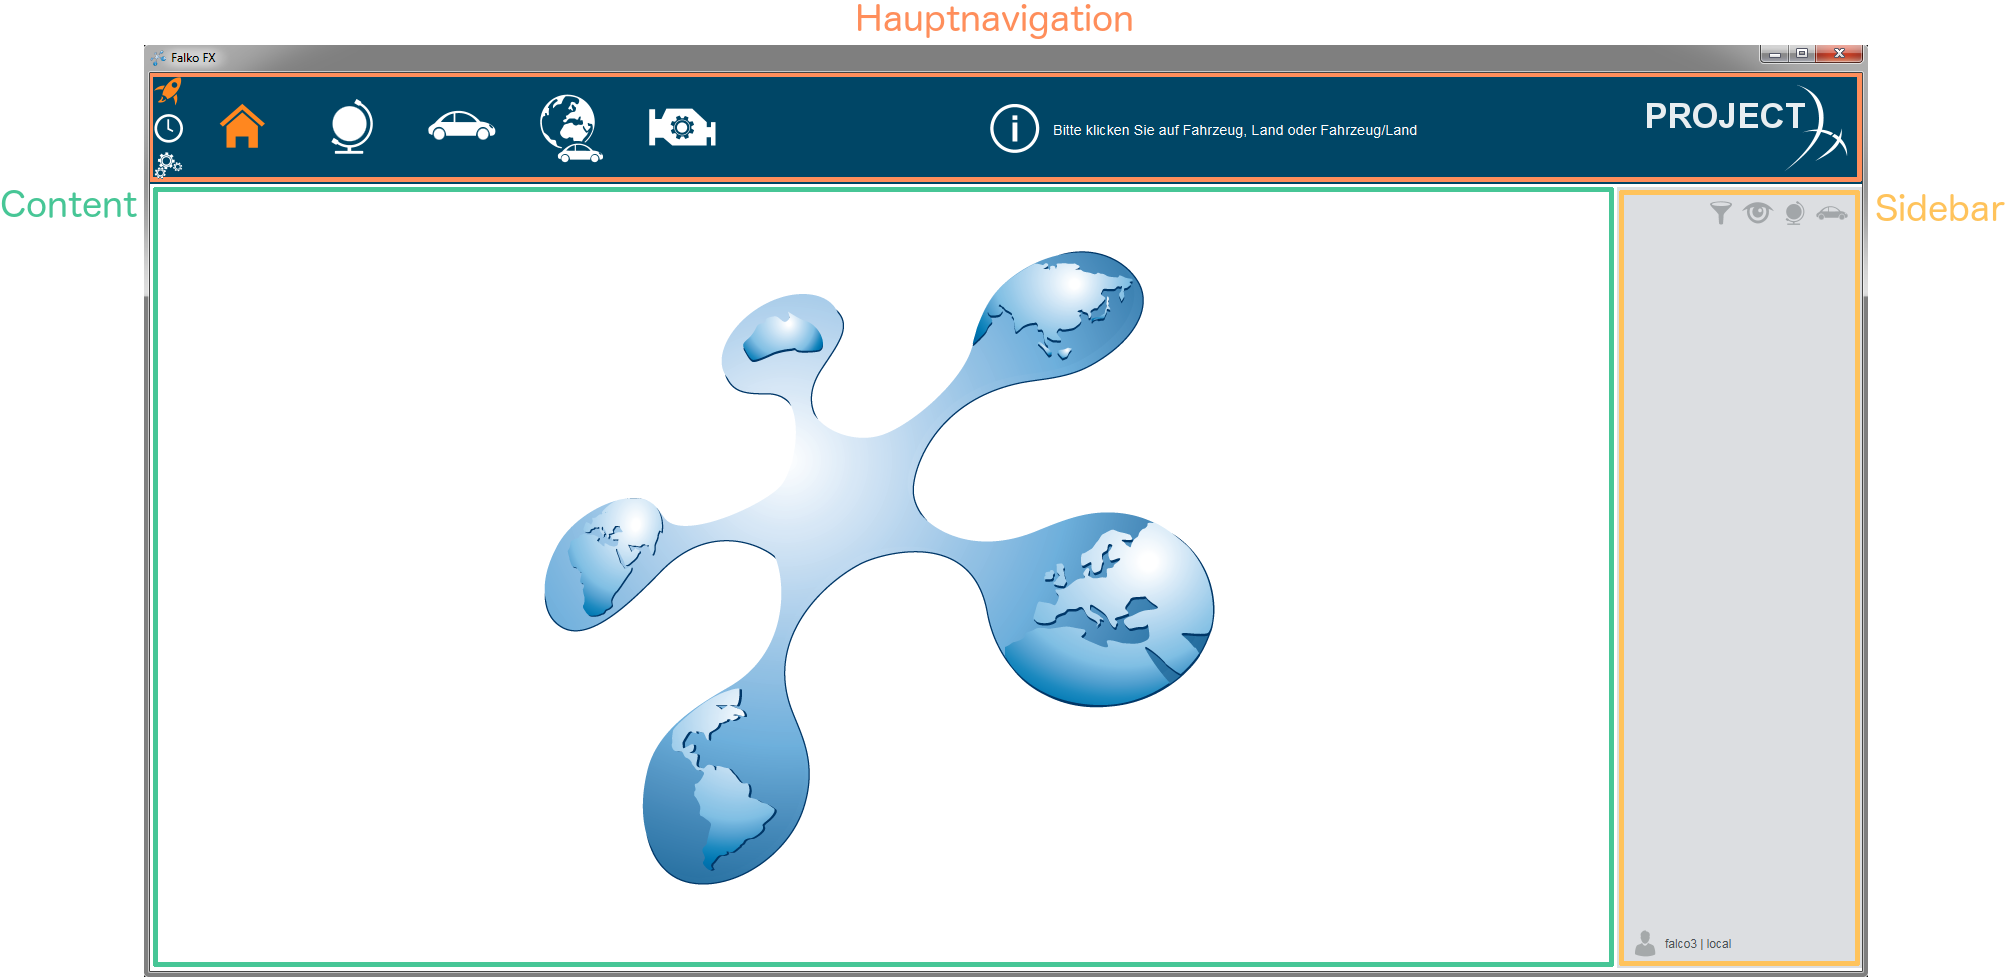
\includegraphics[width=0.8\textwidth]{grafiken/areas.png}
 \caption{Bereiche in FalkoFX}
 \label{fig:areas}
\end{figure}
Das Konzept der gemeinsamen Region wird hier durch die verschiedenen Hintergrundfarben realisiert und unterstreicht die unterschiedlichen Funktionalitäten.\par
\heading{Navigation}
Im Navigationsbereich findet sich im initialen Zustand die Hauptnavigation wieder. Durch die Bedienelemente an der linken Seite der Leiste kann zwischen folgenden Funktionen gewechselt werden:
\begin{enumerate}
	\item Hauptnavigation: Wechsel zwischen Standard-Anwendungsfällen und der verschiedenen Ansichten
	\item Versionsvergleich: Navigation für Anwendungsfälle mit Versionsvergleich
	\item Einstellungen: Menü zum Ändern anwendungsspezifischer Einstellungen
\end{enumerate}
\begin{figure}[H]
 \centering
 
\includegraphics[width=0.05\textwidth]{grafiken/ribbon.png}
 \caption{Umschalten der Navigation}
 \label{fig:ribbon}
\end{figure}
Durch die vertikale Orientierung, der geringeren Größe und der Nähe zueinander heben sich die Elemente zum Umschalten der Navigation deutlich von den andren Schaltflächen ab. Wird eines der Elemente angewählt, wird eine Aktion ausgeführt und die Kindelemente, falls vorhanden, werden mittels Animation sichtbar. Die nachfolgenden Elemente der höher liegenden Ebenen werden \enquote{zur Seite geschoben}.\par
\begin{figure}[H]
 \centering
 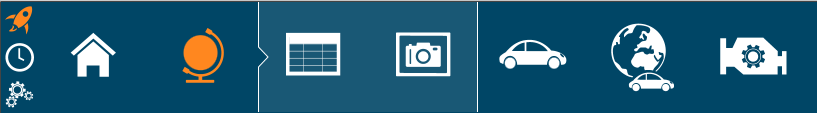
\includegraphics[width=0.85\textwidth]{grafiken/navi.png}
 \caption{Navigationshierarchie}
 \label{fig:navi}
\end{figure}
Die Elemente einer einzigen Navigationsebene benötigen keine weitere Trennung. Durch den Freiraum zwischen diesen ist eine hinreichende Trennung erwirkt. Zwischen den verschiedenen Ebenen wird zusätzlich zu einer Farbabstufung eine weiße Trennlinie eingeblendet, die auf der linken Seite einen angedeuteten Pfeil enthält , der die Navigationshierarchie verdeutlicht. Dazu trägt ebenfalls die bereits erwähnte Animation bei.\par
Das Piktogramm des selektierten Navigationselementes wird orange eingefärbt, um die Orientierung zu gewährleisten. Kann der Nutzer eine bestimmte Interaktion nicht ausführen, erscheint das Icon grau.\par
Durch das Anklicken eines Icons wird der neue Bildschirm angezeigt. Dies geht oft mit dem Laden von Daten einher. Sollten Daten aus der Datenbank geladen werden müssen, wird währenddessen eine Ladeanimation angezeigt. Andernfalls wird der Bildschirm in weniger als 500 Millisekunden angezeigt, wodurch kein weiteres Feedback von Nöten ist. Im Gegenteil: Eine kurz aufblitzende Ladeanimation würde den Anwender eher irritieren als unterstützen.\par
Den Einstieg in jeden auswählbaren Anwendungsfall bietet der Filter. Der Filter besteht aus folgenden Komponenten:
\begin{itemize}
	\item \textbf{Radial-Menü:} Ein rundes Menü, in dem die zu filternden Attribute ausgewählt werden können
	\item \textbf{Multi-Level-Liste:} Eine mehrstufige Liste, aus der Werte zu den Attributen angewählt werden können
	\item \textbf{Filterselektion:} Eine Liste, welche die aktuell ausgewählten Werte gruppiert darstellt und das Abwählen dieser Werte erlaubt
\end{itemize}
\begin{figure}[H]
 \centering
 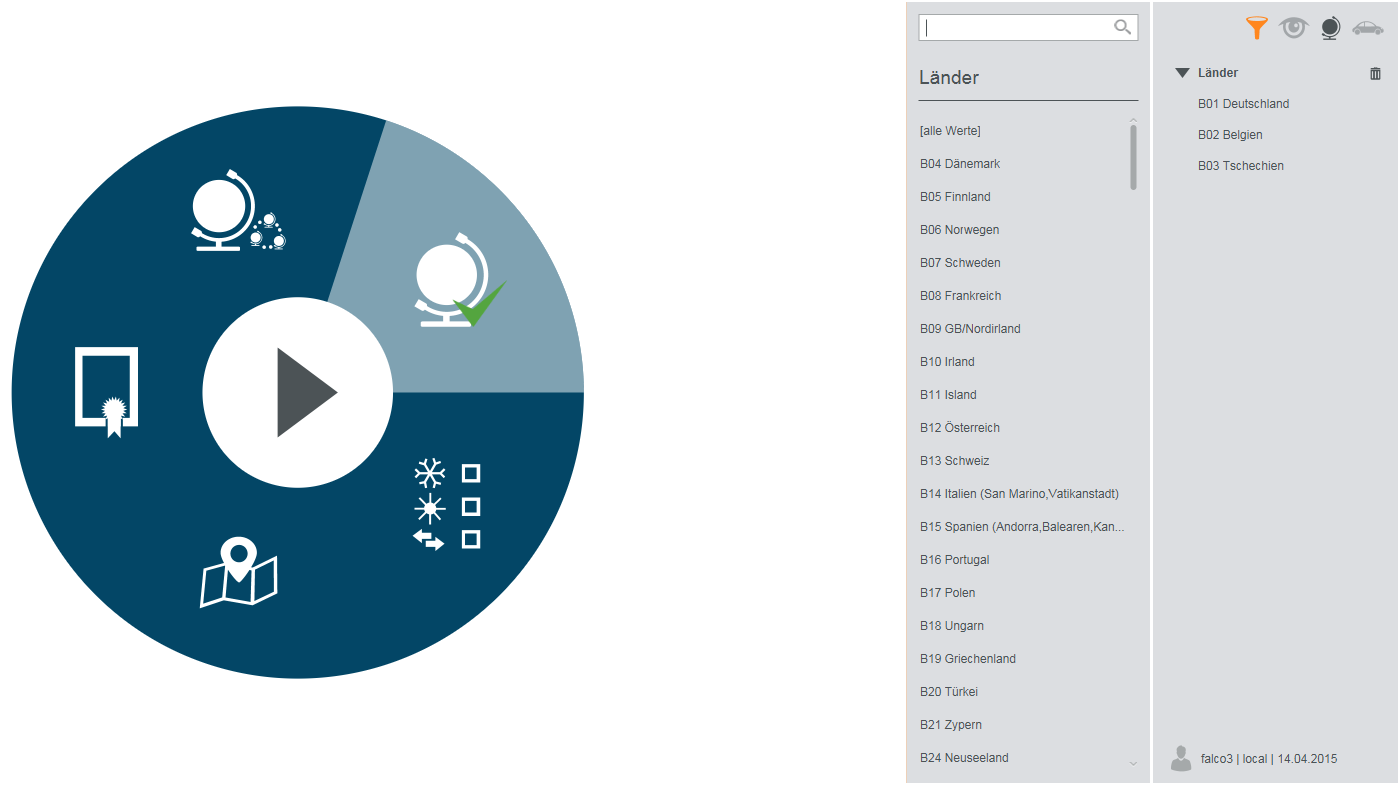
\includegraphics[width=0.5\textwidth]{grafiken/filter_short.png}
 \caption{Beispiel Filter}
 \label{fig:filter}
\end{figure}


\subsection{Übertragung von Touchgesten auf Maussteuerung}
Mit Blick auf den immer stärker werdenden Trend, auch Geschäftsanwendungen auf mobile Geräte zu portieren, soll an dieser Stelle geprüft werden, inwiefern die Touchgesten (vgl. \ref{fig:touchGestures}) auf das Bedienkonzept am Desktop-PC übertragbar sind. Dies soll zum einen zu einer intuitiveren Bedienung mit der Maus beitragen und zum anderen für die Benutzung der Software auf sogenannten Convertibles vorsorgen.\par%Erklärung Convertibles
Der Mauszeiger wird zu diesem Zweck als \enquote{Ersatz} für den Finger auf einem Touch-Display verwendet. Da es nur einen Mauszeiger und eine Maus gibt, ist es technisch gesehen nur möglich, Gesten durchzuführen, die genau einen Finger benötigen. Dies sind \textit{Tap}, \textit{Double Tap}, \textit{Drag}, \textit{Flick} und \textit{Press}. Die \textit{Tap} und \textit{Double Tap}-Gesten entsprechen sowohl von der Durchführung, als auch von der Semantik in der Regel dem einfachen Mausklick bzw. dem Doppelklick. Die \textit{Drag}-Geste ist der Drag\& Drop Aktion der Maus sehr ähnlich. An vielen Stellen jedoch, an denen bei mobilen Anwendungen \textit{Drag}-Gesten verwendet werden würden, wird die Benutzung eines UI-Elements auf dem Desktop-PC mit anderen Mitteln gelöst. Für den \textit{Flick}, auch \textit{Swipe} genannt, existiert kein Pendant im Pensum der normalen Maus- und Tastatur- Interaktion. Dennoch ist es denkbar, eine solche Geste mit einer schnell ausgeführten Drag\& Drop-Aktion zu ermöglichen. Auch der \textit{Press} könnte mit den gegebenen Eingabemitteln umgesetzt werden. Eine solche Aktion ist jedoch in den meisten Fällen nur bedingt intuitiv verwendbar, da keine ähnlichen, dem Nutzer vertrauten, Aktionen für die Maussteuerung existieren.\par


\section{Design}
\subsection{•}
\section{Implementierung} \label{sec:interactionImplementation}
